\documentclass{siproblemset}

\usepackage{multicol}
\usepackage{xcolor}
\usepackage{mathtools}

% SI Session Information
\course{MTH 1321}
\sessionnum{PT2}
\sessiondate{3/3/20}

% Worksheet Information
\title{Practice Test \#2}
\sections{Chapter 3}
\withnamespace

\definecolor{darkred}{RGB}{110,0,0}

%\debugmode

\begin{document}
    \maketitle
    
    \begin{center}
        \framebox{
            \begin{minipage}{\textwidth}
                \begin{center}
                    \textbf{When completing this practice test, do your best to mimic the test environment:}
                \end{center}
                \begin{enumerate}
                    \item Do not use a calculator.
                    \item Try not to use your notes.
                    \item Time yourself, make sure you are completing the problems at a comfortable pace. Remember that you will only get 50 mins for the actual exam (with fewer questions of course).
                \end{enumerate}
                \begin{center}
                    \color{darkred}\textbf{ Please do not share this practice test with anyone else. \underline{Your} commitment \linebreak to SI and reviewing material earned this, not anyone else's.}
                
                    \large \color{blue} When you have finished the practice test, go to answer key folder\linebreak (using the link in your email) to check your answers.
                \end{center}
            \end{minipage}
        }
    \end{center}

    % Limit Definition
    \frq{Use the limit definition of the derivative to show that}
    $$\ddx\left[\frac{x}{x-3}\right]=-\frac{3}{(x-3)^2}$$
    \newpage
    
    % Higher Derivatives
    \mcq{Use any derivative rules that we have introduced up to this point to determine the first and second derivatives of the following functions. \textbf{You do not need to simplify.}}{
        \task $f(x)=5x^2-x^3+2x^{-3}$
        \Smallsp
        \task $H(y)=y^5e^y+\pi$
        \Smallsp
    }

    % Intermediate Derivatives
    \mcq{Use any derivative rules that we have introduced up to this point to determine the first derivatives of the following functions. \textbf{You do not need to simplify.}}{
        \task $g(x)=(3x-5e^x)^4$
        \Smallsp
        \task $f(x)=e^{x^2-3x}-\cos\left(\ln(1)\right) $
        \Smallsp
        \task $h(t)=\sqrt{-2+\dfrac{2}{3t^2}}$
        \Smallsp
        \task $Q(r)=(1-r)^{1/r}$
        \Normalsp
    }

    % Advanced Derivatives
    \mcq{Find the derivative using the rules we have studied. \textbf{Simplify when possible.}}{
        \task $f(x)=\ln(\sec(x^2))$
        \normalsp
        \task $g(t)=\arccos(t^3)$
        \Smallsp
    }

    % Weird Derivative
    \frq{Suppose $f(1)=1/2$, $f'(1)=4$, $g(1)=1/\sqrt{3}$, $g'(1)=3$. Find $H'(1)$ where}
    $$H(x)=\frac{1-x}{f(x)}-x^3f(x^2)-\arcsin(g(x))$$
    \Largesp
    
    % Implicit
    \frq{Determine $\dddx[y]$ where}
    $$\arccos(y)+\frac{8}{y}=2x^2+12e^x$$
    \newpage
    
    % Limit Def
    \frq{Use the limit definition of the derivative to find the derivative of $f(x)=\sqrt{3x+2}$.}
    \Largesp
    
    % Basic Rules
    \mcq{Use any derivative rules that we have introduced up to this point to determine the first derivative of the following functions. \textbf{You do not need to simplify.}}{
        \task $f(x)=\dfrac{3x^7-5}{2x}$
        \Smallsp
        \task $f(x)=e^{-x}\sqrt{1-e^x}$
        \Smallsp
        \task $g(t)=\arccot(3t^2)$
        \Smallsp
        \task $h(x)=(\csc(x))^x$
        \Normalsp
    }

    % Physics
    \begin{multipartquestion}
        A rock thrown vertically upward from the surface of the moon has a velocity of $24$m/s reaches a height of $s(t)=24t-0.8t^2$ m in $t$ seconds.
        \frq{What is the velocity of the rock at the moment it hits the surface of the moon?}
        \normalsp
        \frq{What is the acceleration due to gravity on the moon?}
        \Normalsp
    \end{multipartquestion}

    % Derivative with Table
    \frq{Use the information given in the chart and the function $H(x)$ below to find $H'(2)$. \textbf{Simplify your answer as much as possible.}}
    \begin{multicols}{2}
        $$H(x)=\dfrac{g(x)}{\ln(f(x))}$$\\
        \begin{tabular}{|c|c|c|c|c|}
            \hline
            $x$ & $f(x)$ & $f'(x)$ & $g(x)$ & $g'(x)$ \\
            \hline
            $2$ & $e^2$ & $\pi$ & $e^3$ & $1/2$\\
            \hline
        \end{tabular}
    \end{multicols}
    \Smallsp

    % Related Rates
    \mcq{A 17ft ladder is leaning against a building. The foot of the ladder is 8ft from the base of the building and it's sliding away from the building at 3ft/s.}{
        \task How fast is the top of the ladder sliding down the wall of the building?
        \task How fast is the area formed by the ladder changing at this instant?
    }
    \newpage
    
    % Derivative Rules
    \mcq{Use any derivative rules that we have introduced up to this point to determine the first derivatives of the following functions. \textbf{You do not need to simplify.}}{
        \task $T(x)=\dfrac3x+\sqrt{-2+x^2}$
        \Normalsp
        \task $f(x)=\cos(x^2)\sin(3x)\sec(e^x)$
        \Normalsp
        \task $g(x)=\arcsec(2x^3)$
        \Normalsp
        \task $h(t)=(1+t)^{1/t}$
        \Normalsp
    }

    % Physics
    \begin{multipartquestion}
        Suppose that the distance an aircraft travels along a runway before takeoff is given by $$D=(10/9)t^2$$ where $D$ is measured in meters from the starting point and $t$ is measured in seconds from the time the airplane begins moving down the runway. The aircraft will become airborne when its speed reaches 200 km/hr.
        \frq{How long will it take for the aircraft to become airborne?\newline Hint: 1 km/hr = $\dfrac{5}{18}$ m/s}
        \Normalsp
        \frq{What distance will the aircraft travel along the runway before it takes off? You do not need to simplify your answer.}
        \Normalsp
    \end{multipartquestion}

    % Derivative with table and graph
    \frq{Use the information give and the function $f(x)$ below to find $f'(2)$. \textbf{Simplify your answer as much as possible.}}
    \begin{multicols}{2}
        $$a(x)=x^3-8x$$
        
        \begin{center}
            \begin{tabular}{|c|c|c|c|c|c|c|}
                \hline
                $x$ & -4 & -2 & 0 & 2 & 4 & 6\\
                \hline
                $b(x)$ & $-7$ & 0 & 2 & 0 & $-\pi$ & 3 \\
                \hline
                $b'(x)$ & $-3$ & $-2$ & 0 & $4$ & $-2$ & $2$\\
                \hline
            \end{tabular}
        \end{center}
    
        \begin{center}
            \mbox{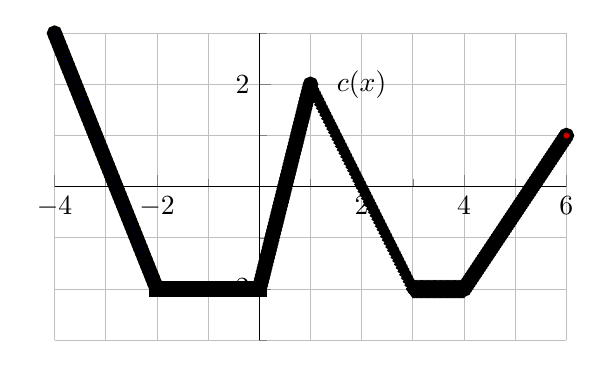
\begin{tikzpicture}[baseline=(current bounding box.north)]
                \begin{axis}[
                x=0.65cm,
                y=0.65cm,
                xmin=-4,
                xmax=6,
                ymin=-3,
                ymax=3,
                grid=both,
                major grid style={line width=.2pt,draw=gray!50},
                minor tick num=1,
                axis x line*=middle,
                axis y line*=middle,
                every axis plot/.append style={ultra thick},
                samples=60
                ]
                \addplot+[black, domain=-4:-2] {-2.5*x-7};
                \addplot+[black, domain=-2:-0] {-2};
                \addplot+[black, domain=0:1] {4*x-2};
                \addplot+[black, domain=1:3] {-2*x+4};
                \addplot+[black, domain=3:4] {-2};
                \addplot+[black, solid, domain=4:6] {3/2*x-8};
                \node at (2,2) {$c(x)$};
                \end{axis}
                \end{tikzpicture}}
        \end{center}
    \end{multicols}
    $$f(x)=\ln(a(x))+b(-2x)c(x)$$
    \Largesp
    
    % Derivatives
    \mcq{Compute the following derivatives. You do not need to simplify your answers.}{
        \task Let $f(x)=12345+\tan^{-1}(x)-\sqrt{x}$. Find $f'(x)$. 
        \Normalsp
        \task Let $g(x)=2x\sec(e^{-x})$. Find $\dddx[g]$.
        \Normalsp
        \task Let $f(t)=\left[\ln(\sin t)\right]^2$. Find $f'(t)$. 
        \Normalsp
        \task If $(x+2y)y=2x-y$, find $\dddx[y]$ at the point (3,1).
    }
    \newpage

    % Implicit differentiation and application
    \mcq{Consider the curve given by the following equation. $$x+\frac{17}{x}=2y^2+12y$$}{
        \task Determine $\dddx[y]$.
        \Largesp
        \task Find all values of $x$ at which the curve has a vertical tangent line.
        \Largesp
    }
\newpage

    % Derivatives from graphs
    \begin{multipartquestion}
        Consider the graph of $f$ shown below.
        \begin{center}
        \mbox{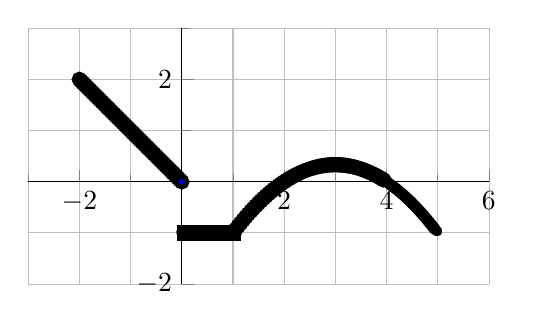
\begin{tikzpicture}[baseline=(current bounding box.north)]
            \begin{axis}[
            x=0.65cm,
            y=0.65cm,
            xmin=-3,
            xmax=6,
            ymin=-2,
            ymax=3,
            grid=both,
            major grid style={line width=.2pt,draw=gray!50},
            minor tick num=1,
            axis x line*=middle,
            axis y line*=middle,
            every axis plot/.append style={ultra thick},
            samples=60
            ]
            \addplot+[black, domain=-2:0] {-x};
            \addplot+[black, domain=0.06:1] {-1};
            \addplot+[black, domain=1:3.94] {-1/3*(x-3)^2+1/3};
            \addplot+[black, domain=4.06:4.94] {-1/3*(x-3)^2+1/3};
            \node at (-2,2) {$\circ$};
            \node at (0,-1) {$\circ$};
            \node at (4,0) {$\circ$};
            \node at (0,0) {\textbullet};
            \node at (5,-1) {\textbullet};
            \end{axis}
            \end{tikzpicture}}
        \end{center}
        \frq{Find all values of $x$ in $[-2, 5]$ such that $f'(x)=0$.}
        \Tinysp
        \frq{Find all values of $x$ in $[-2, 5]$ such that $f'(x)$ is undefined.}
        \Tinysp
        \frq{Find $\lim\limits_{h\to 0}\dfrac{f(h-1)-f(-1)}{h}$.}
        \Tinysp
    \end{multipartquestion}

    % Derivatives
    \mcq{Compute the following derivatives. You do not need to simplify your answers.}{
        \task Let $y=\sin^{-1}(3x)+2^x+\log_2x$. Find $y'(x)$. 
        \Normalsp
        \task Let $y=\sqrt{1+e^{-x}}$. Find $\dddx[y]$.
        \Normalsp
        \task Let $y=\dfrac{\sec x}{\ln x}+x^{-1}\cos(2x)$. Find $y'(x)$.
        \Normalsp 
        \task Let $x^2-xy-3y=3$. Find $\dddx[y]$ at the point $(2,1)$.
    }
    \newpage

    % Extras
    \frq{Find the derivative of $y=\arcsin(x^2)$ using the identity $x=\sin(\sin^{-1}(x))$.}
    \largesp
    
    \frq{Find the derivative of $g(x)=x^{\sin x}$ using an exponential identity.}
\end{document}